\bookchapter{Bab 37: Revolusi Paradigma—Dari “Menulis Kode” ke “Memimpin AI Menulis Kode”}

\chapterintro{Selamat—Anda yang membuka buku ini sedang berdiri di tengah revolusi paradigma profesi. Titik awal revolusi ini adalah satu kalimat seorang programmer di media sosial pada 2025. Terdengar dramatis? Memang begitu adanya.}

\booksection{Kelahiran Vibe Coding: gerakan yang dipicu satu kalimat}

Februari 2025, Andrej Karpathy—ingat nama ini, Anda akan menjumpainya beberapa kali lagi—mengunggah cuitan yang kemudian berulang kali dikutip: “Ada cara baru memprogram yang disebut Vibe Coding—Anda sepenuhnya mengandalkan perasaan (vibes), mengabaikan detail kode, dan membiarkan AI mengerjakan semuanya. Apa yang Anda lihat, itu yang Anda katakan, salin-tempel—intinya yang penting jalan.”

Pernyataan yang terdengar enteng itu sebenarnya menamai dengan tepat pergeseran paradigma yang diam-diam sudah terjadi: manusia tidak lagi menulis kode baris demi baris, melainkan mendeskripsikan maksud dalam bahasa alami, dan AI yang mewujudkannya. Pilihan kata Karpathy sedikit berkelakar, tetapi di baliknya ada wawasan mendalam: setelah kemampuan menghasilkan kode AI melewati ambang tertentu, yang jadi hambatan bukan lagi “bisakah saya menulis baris kode ini”, melainkan “sejelas apa saya memikirkan hal ini”.

\begin{tcbinfo}{Tips: apa itu Vibe?}
Vibe secara harfiah berarti “suasana, perasaan”. Vibe Coding adalah “memprogram dengan mengikuti perasaan sambil memimpin AI”—Anda mendeskripsikan yang diinginkan, AI yang mewujudkan. Ingat istilah ini—ia adalah “akta kelahiran” revolusi ini.

\end{tcbinfo}

Sejak saat itu, makna kata “coding” mulai bercabang: coding tradisional adalah menerjemahkan desain menjadi sintaks; coding baru adalah menerjemahkan maksud menjadi instruksi. Yang pertama menguji jari, yang kedua menguji otak.

Istilah Vibe Coding dengan cepat berubah dari candaan menjadi konsep rekayasa yang serius. Pada pertengahan 2026, ia telah berevolusi dari meme media sosial menjadi metodologi lengkap—mencakup seluruh alur dari ekspresi kebutuhan, manajemen konteks, iterasi verifikasi, hingga penjaminan kualitas. Orang pun menyadari: “mengandalkan perasaan” hanyalah tahap pemula; pemrograman AI yang benar-benar efisien membutuhkan cara berpikir yang sistematis. Dan cara berpikir itulah yang ingin diberikan buku ini kepada Anda.

\booksection{Kondisi 2026: era Agentic Engineering}

Pada Agustus 2026, bidang pemrograman AI telah melewati beberapa iterasi paradigma penting. Vibe Coding adalah percikan awal—tetapi orang segera sadar: sekadar “mengandalkan perasaan” dan mengobrol dengan AI menghasilkan kode yang kualitasnya sangat tidak stabil—sekali memukau, sekali berantakan. Maka paradigma berevolusi: dari pemrograman percakapan sederhana, menuju rekayasa Agent yang terstruktur.

Lagi-lagi Karpathy, awal 2026 mencetuskan konsep Agentic Engineering. Berbeda dengan Vibe Coding yang “bilang lalu jadi”, Agentic Engineering menekankan: beri AI satu tujuan, biarkan ia merencanakan langkah, memanggil alat, memverifikasi hasil, dan mengoreksi secara iteratif secara mandiri. AI bukan lagi sekadar generator kode, melainkan agen (Agent) yang bisa mempersepsi lingkungan, mengambil keputusan, dan menjalankan aksi.

Pergeseran ini membawa tiga perubahan kunci:

\begin{enumerate}
  \item Mode interaksi berubah: dari "tanya-jawab satu kali" menjadi "tetapkan tujuan lalu beri keleluasaan".
  \item Hasil kerja berubah: dari "sepotong kode" menjadi "satu proyek lengkap".
  \item Peran manusia berubah: dari "memeriksa kode baris demi baris" menjadi "mendefinisikan batas, memverifikasi hasil".
\end{enumerate}

Angka tidak berbohong: pada versi Cursor 3 yang dirilis April 2026, tingkat penggunaan mode Agent untuk pertama kalinya melampaui mode penyelesaian Tab—menandakan pengembang telah beralih besar-besaran ke cara kerja ini. Sementara Claude Code, alat pemrograman AI bawaan terminal, pada pertengahan 2026 telah mencapai skala pendapatan tahunan 2,5 miliar dolar AS. Grafik tren berikut memberi Anda gambaran momen persilangan itu:

\begin{center}
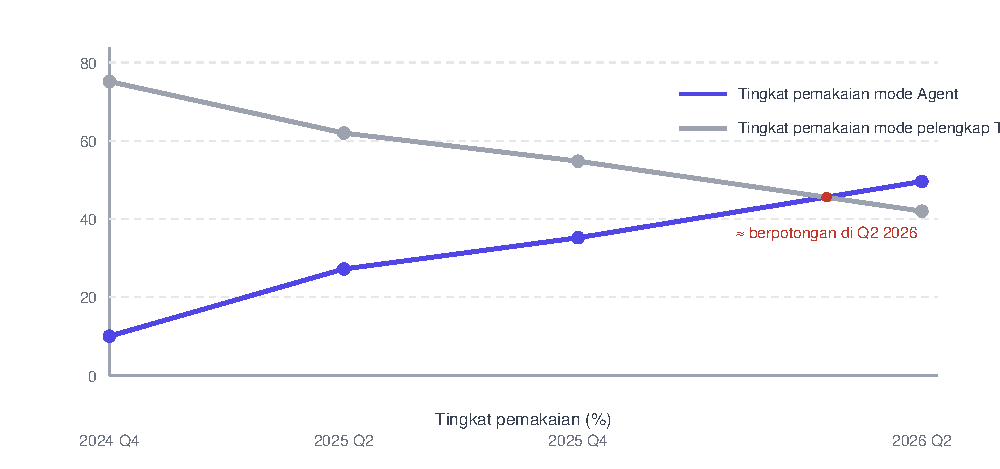
\includegraphics[width=0.92\linewidth]{figures/fig-di-san-shi-qi-zhang-1}
\\[2pt]\small Gambar 1: Tren perubahan tingkat penggunaan mode interaksi pemrograman AI (estimasi berdasarkan data riset industri; Q2 2026 mode Agent melampaui penyelesaian Tab)
\end{center}

Tapi jujur saja: perubahan alat dan model hanyalah permukaan. Entah Anda memakai Cursor atau Claude Code, entah model dasarnya GPT-5 atau Claude 4.5, praktisi pemrograman AI yang sukses semuanya mengikuti metodologi dasar yang sama. Inilah yang akan diajarkan panduan ini kepada Anda.

\booksection{Perubahan kognitif inti: dari Coder ke Conductor}

Pendidikan pemrograman tradisional mengajarkan cara menjadi seorang Coder—memahami sintaks, menghafal API, men-debug kesalahan logika. Di era pemrograman AI, peran ini sedang didefinisikan ulang. Anda tidak perlu lagi menulis setiap baris kode dengan tangan, tetapi Anda perlu menjadi “komandan” (Conductor): mendefinisikan medan, menetapkan aturan, membagi tugas, memverifikasi hasil.

Inti pergeseran ini bukan pada “bisakah Anda menulis kode”, melainkan pada “bisakah Anda memikirkan dengan jelas apa yang akan dikerjakan”. Seorang komandan yang ulung belum tentu prajurit terbaik, tetapi ia harus paling paham tujuan pertempuran, medan, dan penempatan kekuatan. Demikian pula, praktisi pemrograman AI yang ulung belum tentu menguasai detail sintaks setiap bahasa pemrograman, tetapi ia harus paling paham tujuan proyek, batasan arsitektur, dan standar kualitas.

Tabel ini layak Anda baca dua kali—ia merangkum seluhuh isi perubahan peran ini:

\begin{center}
\begin{tabularx}{\linewidth}{|X|X|X|}
\hline
\textbf{Dimensi} & \textbf{Coder tradisional} & \textbf{Komandan AI (Conductor)} \tabularnewline
\hline
Keterampilan inti & Hafalan sintaks, pemanggilan API, debugging & Definisi kebutuhan, manajemen konteks, penilaian verifikasi \tabularnewline
Cara kerja & Menulis kode baris demi baris & Mendeskripsikan maksud, memeriksa hasil \tabularnewline
Pengendalian kualitas & Yang ditulis sendiri, sudah tahu isinya & Memverifikasi keluaran AI lewat pengujian dan tinjauan \tabularnewline
Tuntutan pengetahuan & Menguasai bahasa/kerangka kerja tertentu secara mendalam & Memahami lanskap teknologi secara luas, logika bisnis secara mendalam \tabularnewline
Lokasi hambatan & Kecepatan menulis kode dan hafalan sintaks & Kejernihan berpikir dan kemampuan mengekspresikan \tabularnewline
Sumber kesalahan & Kesalahan sintaks, kelalaian logika & Kebutuhan tidak jelas, konteks kurang \tabularnewline
\hline
\end{tabularx}
\end{center}

\begin{center}\small\color{gray}Perbandingan dimensi kemampuan Coder tradisional dan Komandan AI\end{center}

Ini sama sekali tidak berarti pengetahuan pemrograman tidak penting. Justru sebaliknya: hanya ketika Anda bisa membaca kode yang ditulis AI, Anda bisa memeriksa dan memperbaikinya secara efektif; hanya ketika Anda memahami struktur data dan algoritma, Anda bisa menilai apakah solusi AI masuk akal. Cadangan pengetahuan menentukan “batas komando” Anda—tetapi peran pengetahuan berubah dari “alat pelaksana” menjadi “dasar penilaian”.

\booksection{Mengapa metodologi lebih penting daripada alat}

Alat beriterasi setiap tiga bulan, metodologi berevolusi setiap tiga tahun. Menguasai cara memakai sebuah alat bisa usang dalam tiga bulan; menguasai satu pola pikir tetap terpakai tiga tahun kemudian.

Banyak orang saat mulai belajar pemrograman AI langsung bertanya “alat mana yang terbaik” “model mana yang terkuat”. Pertanyaan itu bukan tidak penting—tetapi prioritasnya salah. Lanskap alat Agustus 2026 sudah sama sekali berbeda dari Agustus 2025—Trae, Qoder, dan lainnya naik-turun; Cursor berubah dari plugin menjadi IDE mandiri lalu berevolusi ke Cursor 3; Claude Code berubah dari proyek eksperimental menjadi pilihan utama pemrograman terminal. Namun di balik perubahan dahsyat itu, prinsip berpikir yang diikuti praktisi sukses nyaris tidak berubah.

Karena itulah buku ini tidak membuang halaman untuk mengajarkan operasi spesifik satu alat—materi seperti itu akan usang begitu selesai ditulis. Sebaliknya, seluruh fokus buku ini ada pada metodologi berpikir yang teruji: bagaimana memikirkan kebutuhan, bagaimana berkomunikasi dengan AI, bagaimana memverifikasi hasil, bagaimana terus beriterasi. Setelah menguasai metodologi ini, alat apa pun bisa Anda kuasai dengan cepat; kalau hanya belajar operasi alat, ganti alat harus mulai dari nol lagi.

\begin{tcbinfo}{Penenang untuk pembaca pemula}
Jika Anda benar-benar pemula, jangan takut dengan kata “metodologi”. Metodologi bukan filsafat abstrak—ia adalah panduan operasional “bagaimana berpikir saat menghadapi masalah”. Ibarat belajar memasak: Anda bisa mengikuti resep langkah demi langkah (operasi alat), tetapi koki sejati memahami “mengapa bumbunya begini” “bagaimana mengendalikan api” (metodologi). Buku ini dimulai dari konsep paling dasar, setiap prinsip dilengkapi contoh perbandingan konkret—memastikan Anda tidak hanya memahami “apa”, tetapi benar-benar menguasai “bagaimana”.

\end{tcbinfo}

\begin{tcbpractice}{Ayo praktik: ambil "foto peran" Anda saat ini}
Ambil selembar kertas, tulis jawaban atas tiga pertanyaan: (1) Bagaimana Anda sekarang memakai AI untuk membantu menulis kode (jika pernah)? (2) Anda lebih mirip “Coder” atau “komandan” pada tabel di atas? (3) Bagaimana Anda ingin diri Anda tiga bulan lagi mendeskripsikan cara kerjanya? Setelah ditulis, selipkan di buku ini—baca Bab 47 lalu kembali melihatnya. Anda akan sadar perubahannya lebih cepat dari perkiraan.

\end{tcbpractice}

\begin{tcbsummary}{Ringkasan bab ini}
\begin{itemize}
  \item Pada 2025 Karpathy menamai revolusi pemrograman AI "Vibe Coding": dari menulis kode baris demi baris, menjadi mendeskripsikan maksud dalam bahasa alami
  \item Pada 2026 berevolusi ke Agentic Engineering: beri tujuan, beri keleluasaan, AI merencanakan dan mengeksekusi sendiri, manusia memverifikasi hasil
  \item Tingkat penggunaan mode Agent Cursor 3 untuk pertama kalinya melampaui penyelesaian Tab; pendapatan tahunan Claude Code mencapai 2,5 miliar dolar AS
  \item Peran baru Anda adalah Conductor (komandan): mendefinisikan medan, menetapkan aturan, membagi tugas, memverifikasi hasil
  \item Alat berganti setiap tiga bulan, metodologi baru berevolusi setiap tiga tahun—pelajarilah metodologi, bukan sekadar operasi
\end{itemize}

\end{tcbsummary}
